% vim: set sts=4 et :
\documentclass[aps,prd,reprint,nofootinbib,preprintnumbers]{revtex4}

\usepackage[T1]{fontenc}
\usepackage[utf8]{inputenc}

\usepackage{amsfonts}
\usepackage{amsmath}
\usepackage{graphicx}
\usepackage[svgnames]{xcolor}
\usepackage{hepparticles}
\usepackage{hepnicenames}
\usepackage{hepunits}
\usepackage{hyperref}
\usepackage{graphicx}
\usepackage{epstopdf}

%% Shortcuts %%
\newcommand{\aver}[1]{\langle #1 \rangle}
\newcommand{\dual}[1]{\tilde{#1}}
\newcommand{\est}[1]{\widehat{#1}}
\newcommand{\ie}{\textit{i.e.}}
\newcommand{\nuvec}{\vec{\nu}}
\newcommand{\order}[1]{\mathcal{O}\left({#1}\right)}
\newcommand{\refapp}[1]{app.~(\ref{app:#1})}
\newcommand{\refeq}[1]{eq.~(\ref{eq:#1})}
\newcommand{\reffig}[1]{fig.~(\ref{fig:#1})}
\newcommand{\refsec}[1]{sec.~(\ref{sec:#1})}
\newcommand{\reftab}[1]{tab.~(\ref{tab:#1})}
\newcommand{\rmdx}[1]{\mbox{d} #1 \,} % differential
\newcommand{\thvec}{\vec{\vartheta}}
\let\oldtheta\theta
\renewcommand{\theta}{\vartheta}
\let\eps\varepsilon
\newcommand{\vecest}[1]{\widehat{\vec{#1}}}
\newcommand{\wwhat}[1]{\widehat{\widehat{#1}}}

\DeclareMathOperator{\cov}{Cov}
%\DeclareMathOperator{\skew}{Skew}
\DeclareMathOperator{\kurt}{Kurt}

%% Draft Macros %%
\newcommand{\todo}[1]{{\color{red}\bf ToDo: #1}}
\newcommand{\danny}[1]{{\color{purple}#1}}
\newcommand{\fred}[1]{{\color{brown!85!black}#1}}
\newcommand{\nico}[1]{{\color{green!85!black}#1}}
\newcommand{\citeneeded}{{\color{red}\bf [cite needed]}}

\begin{document}

\allowdisplaybreaks

\preprint{SI-HEP-2014-17}
\title{Extracting Angular Observables without a Likelihood\\and Applications to Rare Decays}
\author{Frederik Beaujean}
\email{frederik.beaujean@lmu.de}
\affiliation{C2PAP, Universe Cluster, Ludwig-Maximilians-Universit\"at M\"unchen, Garching, Germany}
\author{Marcin Chrz\k{a}szcz}
\email{mchrzasz@cern.ch}
\author{Nicola Serra}
\email{nicola.serra@cern.ch}
\affiliation{Physik-Institut, Universit\"at Z\"urich, Z\"urich, Switzerland}
\author{Danny van Dyk}
\email{vandyk@tp1.physik.uni-siegen.de}
\affiliation{Theoretische Physik 1, Naturwissenschaftlich-Technische Fakult\"at,
Universit\"at Siegen, Siegen, Germany}

\begin{abstract}
In this letter we study how to obtain a set of angular observables
$\{S_i\}$ that arise in a generic multi-body process without the need
to carry out a likelihood fit of an angular distribution to the
measured events. Instead, we present a method that only relies on
orthogonality of angular functions, and estimation of integrals
by means of Monte Carlo techniques. Beyond providing estimators
for central values and uncertainties, we provide means to determine
the correlation between all angular observables. We show that detector
acceptance effects can be accounted for in the analysis.
\end{abstract}

\maketitle

\section{Introduction}
\label{sec:intro}

The initial motivation for studying what we wish to call the \emph{Method of Moments}
is the determination of angular observables in the rare decay FCNC-mediated decay
$\bar{B}\to \bar{K}^*(\to \bar{K}\pi)\ell^+\ell^-$. However, we emphasize that
the method we describe in this letter is general, and it applies to arbitrary
decay or scattering processes. We find a previous work \cite{Dighe:1998vk}
advocates this method chiefly for the determination of angular observables in non-leptonic
$B$ decays, but also mentions the applicability to semileptonic decays. We improve
upon this previous work by studying correlations between the angular observables,
and sources of systematic uncertainties. Moreover, we will show that the method
at hand has two benefits over the usual approach based on likelihood fits. To wit:
\begin{enumerate}
    \item Likelihood fits have convergence problems for a small number of
        events, and can require reparametrizations and/or approximations
        for a successful fit to the signal PDF, see e.g. \cite{Egede:2008uy}.
        The method of moments has no such convergence problems.
    \item The results of likelihood fits suffer from systematic uncertainties
        and systematic bias (see e.g. \cite{Egede:2008uy}), especially in but not limited
        to cases in which the PDFs do not faithfully model the underlying physics. We will
        show that the method of moments does not suffer a very particular type of
        mismodelling that arises from introducing a cutoff in a partial wave expansion.
    \item Using the method of moments, the joint probability distribution of the
        angular observables converges towards a multivariate Gaussian distribution.
        This allows an easy transfer of correlation information from the experiments to
        interested theorists.
\end{enumerate}


We continue with basic definitions that pertain to angular observables, and our
results in the subsequent sections. Let $\thvec = (\theta_1, \dots \theta_N)$ denote the set of all
angles, and let $\nuvec = (\nu_1, \dots \nu_M)$ denote the set of all
other non-angular kinematic variables needed to fully specify the
final state of the process under study. For example, $\nuvec$ may
include invariant masses or center-of-mass energies. We define an
angular observable $S_i$ as a coefficient in the probability density
function (PDF) of the process by means of
\begin{align}
    \label{eq:def-P}
    P(\nuvec, \thvec) \equiv \sum_i S_i(\nuvec) \times f_i(\thvec)\,.
\end{align}
Here, the dependence on the $n$ decay angles $\thvec$ has been
explicitly factored out in terms of the angular functions
$\{f_i(\thvec)\}$. We assume there exists a dual basis of functions
$\{\dual{f}_i(\thvec)\}$ such that the orthonormality relations
\begin{equation}
    \label{eq:def-ortho-rel}
    \int_\Omega \rmdx{^N \theta} \dual{f}_i(\thvec) f_j(\thvec)  = \delta_{ij}
\end{equation}
hold with $\Omega$ representing the full angular phase space relevant
to the process.  For particle decays, $P$ is generally expressed in
terms of the fully differential decay width,
\begin{align}
    \label{eq:def-P-decay}
    P(\nuvec, \thvec) \equiv \frac{1}{\Gamma}\frac{\rmdx{^{N+M}\Gamma}}{\rmdx{\nu_1} \dots \rmdx{\nu_M} \rmdx{\theta_1} \dots \rmdx{\theta_N}}\,,
\end{align}
where $\Gamma$ is the total decay width. For a scattering process, one can similarly use
\begin{align}
    \label{eq:def-P-scattering}
    P(\nuvec, \thvec) \equiv \frac{1}{\sigma}\frac{\rmdx{^{N+M}\sigma}}{\rmdx{\nu_1} \dots \rmdx{\nu_M} \rmdx{\theta_1} \dots \rmdx{\theta_N}}\,,
\end{align}
where the total cross section $\sigma$ is used for the
normalization. Since the determination of the total decay width or
total cross section can be quite difficult, we emphasize that
different normalizations for $P$ can be used.  For instance, the total
decay width (or cross section) of the process of interest can be
replaced by the corresponding quantity of a control-channel
process. This change of normalization is equivalent to a linear rescaling of
the angular observables $\lbrace S_i\rbrace$; thus ratios or similar suitable combinations
of the angular observables are invariant.\\

% Our method is closely related to Pearson's method of moments
% \citeneeded{}. One draws samples from a PDF $P(x | \nuvec)$ that
% depends on parameters $\nuvec$. Then one approximates the population
% (central) moments $x^k$ by the sample moments
Our method is an extension of the classical method of moments with
orthogonal functions~\cite[sec. 8.2]{James:2006zz}. The only difference
is that conventionally the angular functions are assumed
\emph{self-dual}, $\dual{f}_i = f_i$. However, it suffices that the
system of angular functions $\{f_i(\thvec)\}$ \emph{can} be transformed into
an orthonormal basis. It turns out to be much more convenient to work
in the basis natural to each process but the statistical properties
are equivalent for both approaches provided that one replace $f_i \to
\dual{f}_i$ appropriately. Using the ansatz
\begin{equation}
  \label{eq:dual-ansatz}
  \dual{f}_i = \sum_{j} a_{ij} f_j \,,
\end{equation}
the dual basis needs to be worked out case by case through solving the
linear system of equations (\ref{eq:def-ortho-rel}). For a selection
of hadron decays with a $b$ quark in the initial state and two leptons
in the final state, we list the dual bases in a series of appendices
\ref{app:btokll} through \ref{app:lambdabtolambdall}. Note that a
similar analysis was done in~\cite{Dighe:1998vk} for the decays $B \to
J/\psi \phi$ and $B \to J/\psi K^{*}$.

In the remainder of this letter we discuss how to obtain an angular
observable $S_i(\nuvec)$ in an experimental setup where each recorded
event is (approximately) distributed according to $P$.  We establish
the statistical basics in section \ref{sec:sample-based-det}. Section
\ref{sec:systematics} is dedicated to the impact of systematic effects
such as mismodeling the underlying physics or detector acceptance
effects. Numerical studies for one uni-angular and one triple-angular
distribution are provided in section \ref{sec:numerics}. In a series
of appendices we provide the orthonormal bases of angular functions
relevant to several rare $b$ decays.



\section{Sample-Based Determination}
\label{sec:sample-based-det}

The orthonormality relations \refeq{def-ortho-rel} imply that a single angular observable $S_i$
can be projected out of the full PDF $P$ by means of
\begin{equation}
    \label{eq:det-Pi-analytical}
    S_i(\nuvec) = \int_{\Omega} \rmdx{^N \theta}  P(\nuvec, \thvec) \dual{f}_i(\thvec)\,.
\end{equation}
where $\lbrace \dual{f}_i \rbrace$ denotes a \emph{dual basis} of angular functions. In general, $\lbrace \dual{f}_i \rbrace$ may differ from $\lbrace f_i \rbrace$. This is the
case for our selection of applications in appendices \ref{app:btokll} through \ref{app:lambdabtolambdall}.\\

It is sensible to refer to the angular observable $S_i$ as the
\emph{$f_i$-moment} of the PDF $P$.  We emphasize that a relation of
type \refeq{det-Pi-analytical} holds for any combination of a density
written as in \refeq{def-P} and an orthonormal basis of angular
functions $\lbrace f_i \rbrace$; \ie, there is no unique
basis of angular functions. For the proof we refer to ref. \cite{Dighe:1998vk}.\\

Integration over the non-angular variables yields
\begin{equation}
    \langle S_i\rangle
    \equiv \int \rmdx{^M \nu} S_i(\nuvec)
    = \int \rmdx{^M \nu} \left[\int_{\Omega} \rmdx{^N \theta} P(\nuvec,\thvec) \dual{f}_i(\thvec) \right].
\end{equation}
The remainder of this section describes the method of moments, in
which we replace the analytical integration by Monte Carlo (MC)
estimates.  The central tenet of MC integration is the fact that the
expectation value $E_P[g]$ of some function $g(x)$ under the
probability density $P(x)$,
\begin{equation}
    E_P[g] \equiv \int \rmdx{x} P(x) g(x),
\end{equation}
can be approximated by the consistent and unbiased
estimator $\est{E_P[g]}$~\cite[sec. 8.2]{James:2006zz}
\begin{equation}
    \label{eq:mc-id}
    E_P[g] \to \widehat{E_P[g]} \equiv \frac{1}{K} \sum_{k=1}^K g(x^{(k)}) \,,\,    x^{(k)} \sim P
\end{equation}
due to the strong law of large numbers for $K \to \infty$, assuming
that the variates $x^{(k)}$, $k = 1, \dots, K$, are distributed as
$P$.
Throughout this letter we denote all MC estimators with a wide hat.\\


Application of \refeq{mc-id} then yields
\begin{equation}
    \langle S_i\rangle \to \widehat{\langle S_i\rangle} = \frac{1}{K} \sum_{k=1}^{K} \dual{f}_i(x^{(k)})\,.
\end{equation}
It is often of interest to obtain observables integrated over certain
bins of $\nuvec$. We define
\begin{align}
    \langle S_i\rangle_{\vec{a},\vec{b}}
    & \equiv \int_{\vec{a}}^{\vec{b}} \rmdx{^M \nu} S_i(\nuvec)\\
    & = \int_{\vec{a}}^{\vec{b}} \rmdx{^M \nu} \left[\int_{\Omega} \rmdx{^N\theta} P(\nuvec,\thvec) \dual{f}_i(\thvec)  \right]\\
    & = \int \rmdx{^M \nu} \left[\int_{\Omega} \rmdx{^N\theta}  P(\nuvec,\thvec) \dual{f}_i(\thvec)
        \mathbf{1}(\vec{a} \le \nuvec \le \vec{b})\,
        \right],
\end{align}
where the argument of the indicator function $ \mathbf{1}(\vec{a} \le
\nuvec \le \vec{b})$ is to be interpreted componentwise.
Application of \refeq{mc-id} immediately yields
\begin{equation}
    \label{eq:bin-importance}
    \widehat{\langle S_i\rangle_{\vec{a},\vec{b}}}
    = \frac{1}{K} \sum_{k=1}^{K} \dual{f}_i(x^{(k)})         \mathbf{1}(\vec{a} \le \nuvec \le \vec{b})\,.
\end{equation}
For notational simplicity, let us forget about the $\nuvec$
integration and consider only $S_i$. In the limit $K \to \infty$, the
central limit theorem (CLT) implies that the random vector
\begin{equation}
  \label{eq:angular-obs-vec}
  \vecest{S} \equiv (S_1, \dots, S_i\,,
  \dots)
\end{equation}
follows a multivariate Gaussian distribution $\mathcal{N}( \vec{S},
\widehat{\Sigma})$ centered on the true value $\vec{S}$ with the
covariance $\widehat{\Sigma}_{ij}$ estimated as
\begin{equation}
    \cov[S_i,S_j] \to \est{\cov}[{S}_i, {S}_j]
        = \frac{1}{K - 1} \sum_{k=1}^{K} \big[\dual{f}_i(x^{(k)}) - \est{ S_i}\big]\,\big[\dual{f}_j(x^{(k)}) - \widehat{ S_j}\big]\,.
\end{equation}
In our physics applications, the parameter space is compact and each
$\dual{f}_i$ is bounded. Hence the requisites for the most basic
version of the CLT to hold --- finite mean and covariance of
$\dual{f}_i$ --- are automatically satisfied.  We would like to
emphasize that the sample covariance should \fred{``Should'' as in it
  does in practice? Reference toy studies below} rapidly converge
towards the true covariance matrix.  We propose to declare convergence
\fred{I'd prefer: check that skewness and kurtosis are sufficiently
  small} once estimators for skewness and kurtosis are sufficiently
small,

\begin{equation}
    \est{\operatorname{Skew}}[S_i,S_j] \leq B_S\,\,\text{ and }\,\,\est{\kurt}[S_i,S_j] \leq B_K\,.
\end{equation}
where the limits $B_S$ and $B_K$ should be determined from process-specific dedicated toy studies.\\

Compared to the usual maximum-likelihood approach, we find for the method of moments:
\begin{enumerate}
  \item The angular observable ${S_i}$ can be determined
  independently of any other observable ${S_j}$. It is therefore
  much more robust to physics assumptions needed to define the full
  likelihood. In particular, this means one does not have to be
  specific regarding the form of new-physics contributions; in fact,
  one does not even need to be able to explicitly formulate the
  likelihood at all.
\item It is superior for a small number of samples $N$. Likelihood
  fits tend to be numerically unstable if lots of parameters need to
  be estimated from sparse data. This is more severe if the mode of
  the likelihood is near the boundary of the physically allowed
  region.\fred{Is there some LHCb note we could cite?} In many of the
  decays of interest, there are only say dozens of events recorded.
\item The estimate is unbiased for any $N$. In contrast, the
  maximum-likelihood estimate has a bias of order
  $1/N$~\cite{Cox:1968}. In practice, one should keep in mind the
  bias-variance trade-off: it is a well known phenomenon that removing
  the bias usually leads to an increase in variance of the sampling
  distribution of the estimator~\cite[sec. 7.3]{James:2006zz}. From a
  Bayesian decision-theory point of view, both contribute similarly to
  the expected loss associated with deciding on just one value of the
  unknown parameter. It is therefore highly questionable to reduce
  only the bias~\cite[sections 13.8,17.2]{jaynes:2003}. In fact, for
  the results discussed below in \refsec{numerics}, the likelihood
  fits --- if they converge --- produce uncertainties (10--15)\%
  smaller than those from the method of moments.
  \item The approximate multivariate Gaussian distribution of $\vecest{S}$
  allows easier and more correct transfer of the information in the
  data to interested theorists for more accurate fits of
  standard-model and new-physics parameters \citeneeded\fred{Our fits
    and others'?} or for more precise predictions of optimized
  observables; e.g.,
  \cite{Egede:2008uy,Egede:2010zc,Bobeth:2010wg,Becirevic:2011bp,
    Bobeth:2012vn,Matias:2012xw,DescotesGenon:2012zf} for definitions
  of such optimized observables in $B\to K^*\ell^+\ell^-$ decays,
  \cite{Faller:2013dwa} for application to the decay $B\to
  \pi\pi\ell^-\bar\nu_\ell$, and \cite{Boeer:2014xx} for observables
  in $\Lambda_b\to\Lambda(\to N\pi)\ell^+\ell^-$). While the
  likelihood also approaches a multivariate Gaussian as $K \to
  \infty$, the two methods differ in their utility as input for
  theorists if $\widehat{\vec{S}}$ is not well
  inside the physical region. For example, suppose there are two
  angular observables that are constrained to a triangular region by
  phase-space or unitarity arguments as \fred{Could add a sketch. It
    is supposed to resemble $A_{\text{FB}},F_L$ for $B \to K^* \ell
    \ell$.}
  \begin{equation}
    \label{eq:constr-ex}
    |S_1| + S_2 \le 1, \, S_1 \in [-1,1],\, S_2 \in [0,1] \,.
  \end{equation}
  It may (and often does) happen in practice that $\widehat{\vec{S}}$
  is close or even outside the allowed region such that a significant
  part of the probability mass covers unphysical values. In a Bayesian
  fit, one would take $\mathcal{N}(\vecest{S} | \vec{S},
  \widehat{\Sigma})$ as the sampling distribution of the ``data'', and
  simply set a uniform prior on the triangle in the $\vec{S}$ plane
  defined by \refeq{constr-ex} to have a well defined problem. This
  could be trivially combined with other independent information in a
  global fit. Someone with a different physics model might have to
  consider a
  different physical region, and could incorporate it just as easily.\\

  For a likelihood fit, the constraint needs to be part of the
  analysis performed by the experimental collaboration, and the
  resulting likelihood as a function of $\vec{S}$ is distinctly not
  Gaussian.  For experimentalists, communicating such a result has
  proved to be challenging due to technical reasons (data formats,
  size etc.) and the fear that theorists misinterprete the many
  nuisance parameters (from control channels, detector calibrations
  etc.) that are also part of the likelihood. This leads to the
  undesirable situation that that only the mode and standard errors
  are reported, and theorists often include the results as independent
  measurements with a Gaussian distribution and disregard the boundary
  problem as well as correlations altogether.

\end{enumerate}



\section{Sources of Systematic Uncertainties}
\label{sec:systematics}

In \refsec{sample-based-det}, we assume that the PDF $P$ describes the underlying physics accurately,
and that the experiment observes each event with perfect accuracy. In order to estimate systematic
uncertainties, we lift these assumptions.

\subsection{Mismodeling due to Contributions by Higher Partial Waves}
\label{sec:systematics:partial-waves}

\begin{figure}
    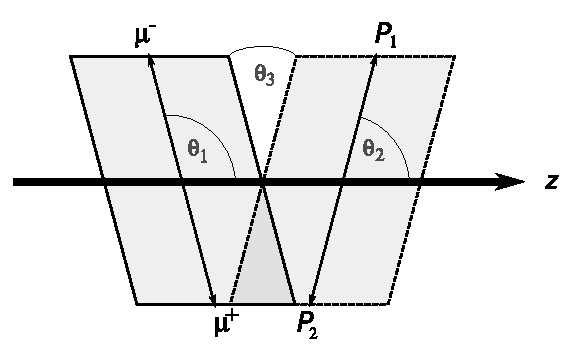
\includegraphics[width=.6\textwidth]{fig-topology.pdf}
    \caption{Decay topology for decays $B\to P_1 P_2 \ell_1 \bar\ell_2$. \label{fig:topology}\fred{We should use the same symbol $\theta$ as in text}}
\end{figure}

In several interesting processes we might only have an approximate
result for $P$.  In this section, we focus on one particular class of
mismodelling of the signal PDF: the angular momentum-cutoff in partial
wave expansions. This mismodelling potentially affects a large number
of decays and scattering processes. For the sake of clarity we take
the interesting class of four-body decays $B\to P_1 P_2 \ell_1
\bar\ell_2$ \fred{How general is this? The plot implies that the
  dimeson and the dilepton do not have a common vertex. But this
  requires an intermediate state, e.g., $K^{*}$}as an
example\footnote{This includes the rare $b\to s$ mediated $B$ decay $B
  \to K\pi\ell^+\ell^-$, and the $V_{ub}$ suppressed decay $B\to
  \pi\pi\ell^+\bar\nu_\ell$. For both examples the PDF $P$ is known in
  the small-width approximation and when assuming a pure $P$-wave,
  resonant final state. An extension to $S-P$ interference has been
  studied for $B\to K\pi\ell^+\ell^-$
  \cite{Blake:2012mb,Becirevic:2011bp}, and for $\bar{B}\to
  \pi\pi\ell^-\bar\nu_\ell$ \cite{Faller:2013dwa}. For a first study
  of $S$, $P$
  and $D$ interference, see \cite{Das:2014sra}}.\\

Within existing analyses, the PDFs of these decays are usually expressed in terms of one or a few
partial waves of the dimeson system. However, the angular momentum of the dimeson system is unbounded
from above, and gives rise to an infinite set of angular observables.\\

For the selected class of decays, we can describe that problem as follows: The PDF $P$ has a fixed dependence on the dilepton
helicity angle $\theta_1$ and the azimuthal angle $\theta_3$. (See also \refapp{btokpill} for details
on the angular distribution.) However, at the level of decay amplitudes the dimeson system can have an arbitrarily
large total angular momentum $j$; only its third component is restricted to $m = -1,0,+1$. \fred{check}
We advocate here that is a sensible procedure to perform an expansion in terms of Legendre polynomials $p_{j}^{(|m|)}$
with respect to the remaining angle $\theta_2$. Using the observables $S_k(\vec{\nu})$, $k=1,\dots,9$, with $\vec{\nu}=(q^2, k^2)$
and as defined in \refapp{partial-waves} \fred{A lot of mixing between appendices C and E}, the expansion reads
\begin{equation}
    S_{k}(\vec{\nu},\cos\theta_2) \equiv \sum_{j} \frac{1}{n_{j,|m|}} S_{k,j}(\vec{\nu}) p_{j}^{(|m|)}(\cos\theta_2)\sin\theta_2\,,
\end{equation}
where the the normalization factor $n_{j,|m|}$ is defined in \refeq{legendre-scalar-product}. Within our
example we have (cf. also \refapp{btokpill})
\begin{equation}
    |m| = \begin{cases}
        0\,, & k = 1,2,6\,\\
        1\,, & k = 3,4,5,7,8,9\,,
    \end{cases}\,.
\end{equation}
The angular observables $S_{k,j}$ defined as coefficients of this expansion in Legendre polynomials
have the merit of a well defined total angular momentum, and thus are physically discriminable.
As a consequence of the orthogonality of the Legendre polynomials, any mismodelling (or rather, lack of modelling of higher
partial-wave observables) \emph{does not affect} the method of moments as discussed in the previous section. To wit,
ignoring further (orthogonal) terms in the PDF cannot affect the mean vector $(\dots, S_k, \dots)$ nor its variance. \fred{yes!}\\

Unfortunately, this benefit on the experimental side is accompanied with a theoretical draw back. Each observable
$S_{k,j}(\vec{\nu})$ consists of an infinite sum of bilinears of partial-wave amplitudes. It remains for theoretical
analyses to estimate or calculate the impact of partial waves beyond the S and P wave contributions.
(For $B\to K\pi\ell^+\ell^-$ a first study has been carried out where contributions up to the D wave are studied \cite{Das:2014sra}).\\

We wish to emphasize, however, that detector acceptance effects systematically affect the expansion for any basis
of angular functions, including the one suggested in this section. The means to cope with this problem are discussed
in the following subsection.


\subsection{Recipe for the Determination of Detector Acceptance Effects}
\label{sec:systematics:acceptance}

The determination of a detector's angular acceptance is generally a difficult
task. Here, we will show a systematic method to estimate its effects
based on both the method of moments and MC simulations of the
detector.\\

In the ideal case, one would have an explicit probabilistic model of
the detector acceptance effects and could thus write down the full
forward model from which the measured events arise. In practice, this
would require much more CPU time than available, and one is therefore
forced to simplify the model. The standard approach is to generate
\emph{true} particle events $\lbrace x_t^{(k)}\rbrace =
\lbrace(\vec{\nu}^{(k)}_t,\vec\theta^{(k)}_t)\rbrace$ from a PDF
assumed to describe the bare physical process, and to propagate those
particles through a detailed simulation of the detector. The
observable traces that the particles leave in the detector are fed
into reconstruction algorithms resulting in the \emph{detector} events
$\lbrace x^{(k)}_d\rbrace = \lbrace(\vec{\nu}^{(k)}_d,
\vec\theta^{(k)}_d)\rbrace$.\fred{What about uncertainty in $\vec{\nu}, \vec{\theta}$? How does it enter the experimental likelihood? And how our method?}\\

As before, we assume the PDF $P$ can be decomposed into $N$ parts with angular observables $\lbrace S_k\rbrace$,
\begin{equation}
    P \equiv P(\vec\nu,\vec\theta | \lbrace S_k \rbrace)\,.
\end{equation}
We denote the estimator of an
observable $S_k$ as $\est{S_k}$, which is affected by the detector acceptance. We assume now that there is a linear relation
between the true angular observables $\lbrace S_k^\text{true}\rbrace$, and the estimators $\lbrace \est{S_k}\rbrace$, \fred{We don't need the $^{\text true}$.}
\begin{equation}
    \label{eq:linear-assumption}
    \est{S_i} = \sum_{j = 1}^N M_{i j} S_j^\text{true}\,.
\end{equation}
This assumption is based on a smooth angular acceptance
function. \fred{Check the LHCb \href{http://inspirehep.net/record/1287929}{paper} on $B \to K \ell \ell$: their
  acceptance (fig. 1) is not smooth due to a cut!} \fred{I don't understand. Need a derivation of why this hinges on smoothness} While this will not be true for
the laboratory frame, smoothness may be recovered in a boosted frame,
e.g. the rest frame of the decaying particle.  In that case, the
matrix $M_{ij}$ can be fully determined through the following steps.
\begin{enumerate}
    \item For fixed $j$, let $S_j^\text{true} = 1$, and $S_k^\text{true} = 0\,\forall k\neq j$.
    \item Draw simulated events $\lbrace x_t^{(k)}\rbrace =
      \lbrace(\vec{\nu}^{(k)}_t,\vec\theta^{(k)}_t)\rbrace$ \fred{don't use $k$ as superscript and subscript} from the PDF $P_j$,
      \begin{equation}
        \label{eq:single-comp}
            P_j \equiv P(\vec\nu,\vec\theta | \lbrace S_j = 1, S_{k\neq j} = 0\rbrace)\,.
        \end{equation}
    \item Use the true events as input for the MC simulation of the detector in order to obtain the detector
        events $\lbrace x^{(k)}_d\rbrace = \lbrace(\vec{\nu}^{(k)}_d,\vec\theta^{(k)}_d)\rbrace$.
    \item Determine the uncorrected observables $\lbrace \est{S_k} \rbrace$ based on the detector
        events $\lbrace x^{(k)}_d\rbrace$. For all intents and purposes, automation of this step is only feasible
        with to the method of moments, since it does not suffer form convergence problems.
    \item By virtue of \refeq{linear-assumption} and step 1, the $j$-th column of $M$ has been determined via
        \begin{equation}
            M_{ij} = \est{S_i}\,.
        \end{equation}
    \item Repeat the above steps for all values of $j$ to determine all columns of $M$.
\end{enumerate}

It remains to invert the relation \refeq{linear-assumption}, so that one can determine the unfolded
angular observables $\lbrace \wwhat{S_k}\rbrace$ as
\begin{equation}
    \wwhat{S_i} = \danny{N_\eps} \left(M^{-1}\right)_{ij} \est{S_j}\,.
\end{equation}
\danny{Here $N_\eps$ is a normalization factor based on the detector acceptance function $\eps$. It emerges
    since the product $P(x) \eps(x)$ is not a PDF; it is not normalized appropriately\footnote{We thank
    X.X\danny{Marcin: Please insert whatshisname} for pointing this out.}. We can determine $N_\eps$ by
    imposing
    \begin{gather}
        1 \equiv \int \rmdx{x} P(x | \lbrace \wwhat{S}_k\rbrace) = N_\eps \sum_{k,j} \left(M^{-1}\right)_{kj} \est{S_j}\int \rmdx{x} f_k(x)\,,\\
        \Rightarrow N_\eps \equiv \frac{1}{\sum_{k,j} \left(M^{-1}\right)_{kj} \est{S_j} \int \rmdx{x} f_k(x)}\,.
    \end{gather}
}

We emphasize that this method hinges on the assumption in \refeq{linear-assumption}\danny{which is well motivated:
the PDF is a linear combination of the basis functions $f_i$, and the moments are therefore a linear
functional of said basis functions. Nevertheless,}
we thus suggest to explicitly
test the linearity. One way of testing involves repeating the previous procedure
with $S_j^\text{true} = 1/z$, $z > 0$. If the linearity assumption holds, one should find
\begin{equation}
    M_{ij}(z) = z \est{S_i}\,,
\end{equation}
for a fixed value of $j$. \fred{This is useless. \refeq{single-comp}
  says: draw from a single component $f_j$. This $f_j$ defines the
  distribution, and whatever factor you put in front of it, you get
  the same distribution of events.}

\danny{In order to better understand the detector aceptance effects, we propose two steps. For the sake of
    clarity of our argument, we assume in the following that the PDF $P$ is expanded in products of
    appropriately chosen Legendre polynomials to some multi-index order $\vec{l}_P^{(0)}$. Similarly,
    moments and detector effects are nominally determined up to some order $\vec{l}_M^{(0)}$, with
    $\vec{l}_M^{(0)} \leq \vec{l}_P^{(0)}$. Here and in the following all comparisons are to be read
    for each compoenent.\\
    For the first step, we remind that the unfolding matrix $M$ depends implicitly on the physical
    PDF $P$. We therefore recommend variation of the order of the expansion of $P$ to $\vec{l}_P \geq \vec{l}_P^{(0)}$
    component-wise. This way one can estimate the mixing of PDF terms of order $\vec{l}_P$ into moments of order $\vec{l}_M^{(0)}$
    or lower.\\
    In a second step, we assume using the nominal expansion of the PDF up to order $\vec{l}_P^{(0)}$.
    With moments of order $\vec{l}_M \geq \vec{l}_M^{(0)}$ one can therefore find the impact of the
    acceptance effects on the mixing of moments of order $\vec{l}_M^{(0})$ and below
    into moments beyond the order of the PDF.
    Our recommendation is not illustrated at the hand of numerical examples, which would necessitate
    access to realistic detector models. The latter are not available to persons outside the
    respective collaborations. The proposed studies are therefore beyond the scope of this work.
}



\section{Toy Studies}
\label{sec:numerics}

In order to study the performance of the proposed method, we simulate measurements for one uni-angular
and one tri-angular decay distribution for various numbers of events. As inputs we use the SM predictions
for the decays $B\to K\ell^+\ell^-$ and $B\to K^*(\to K\pi)\ell^+\ell^-$, respectively. We cover the
$q^2$ ranges $1\GeV^2$ to $6\GeV^2$, and $15\GeV^2$ to to the respective kinematic endpoint, with two
bin widths: $1\GeV^2$ and $0.5\GeV^2$. This is to ensure that a wide spectrum of possible values for
the angular observables.\\

Our finding can be summarized as follows:
\begin{itemize}
    \item In all studied cases we observed not a single bias in the pull distribution of the observable.
        All pull distributions can successfully be fitted to a gaussian distribution. As an example, we
        show the pull distributions for the observables $S_5$ and $S_7$ for a SM-like $B\to K^*\ell^+\ell^-$
        decays in \reffig{pulls}.
    \item We study the absolute uncertainty $\sigma_k(K)$ with respect to the angular observable $S_k$
        as a function of the number of simulated events $K$. As expected for a multivariate gaussian
        distribution, we find that the absolute uncertainty is well fitted by
        \begin{equation}
            \label{eq:unc-on-mean}
            \sigma_k(K) = \frac{\sigma_k(1)}{\sqrt{K}}
        \end{equation}
        with $\sigma_k(1) = \order{1}$, regardless of the absolute size of $S_k$. The latter can best be shown
        for the example of uncertainties of two observables. Taking again $S_5$ ($\simeq 27\%$) and $S_7$ ($\simeq 2\%$)
        for SM-like $B\to K^*\ell^+\ell^-$ decays, we show the absolute uncertainty in \reffig{errors}.
    \item For all toy studies, we produce plots of their skewness and their kurtosis as functions of
        $N$. We find in all cases that the mean skewness and kurtosis converge towards zero.
        \todo{Plot Skewness and Kurtosis for $S_5$ and $S_7$ as functions of the number of simulated events $K$.}
\end{itemize}
We find that all of the above results show consistently that the joint distrbution of the angular observables
converges towards a multivariate Gaussian distribution. We propose to describe the resulting distribution as
a multivariate Gauss when skewness and kurtosis are small enough. The precise targets for these quantities
are subject to the details of the physical analysis, and therefore outside the scope of our work.

\begin{figure}[t]
        \centering
            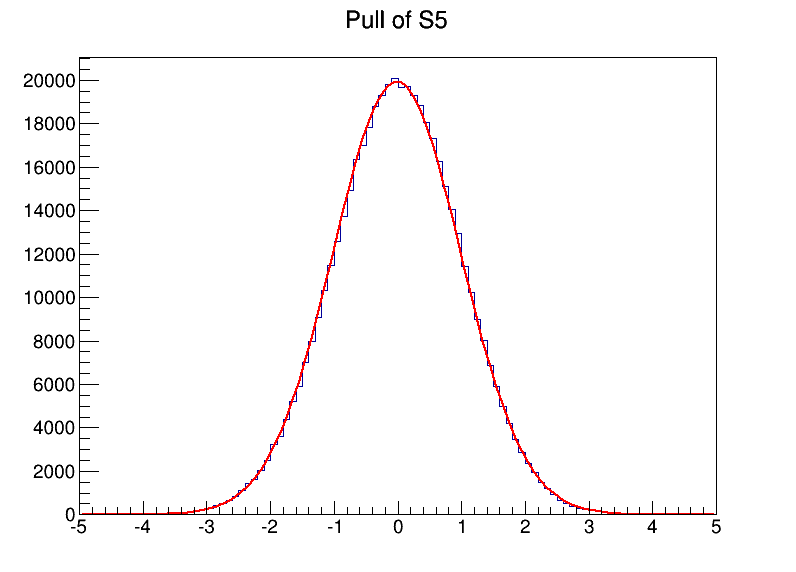
\includegraphics[width=0.45\textwidth]{figs/pull-Q2_5_6_S5_200.png}
            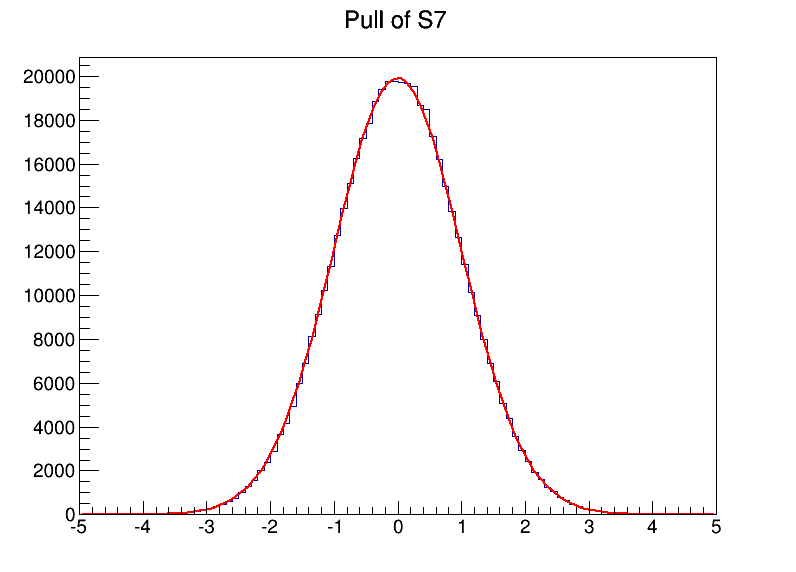
\includegraphics[width=0.45\textwidth]{figs/pull-Q2_5_6_S7_200.png}
        \caption{Pull distribution for the angular observables $S_5$ and $S_7$, extracted from $200$ simulated events of the decay $B\to K^*\ell^+\ell^-$. The red curve represents a fit to a gaussian distribution.}
        \label{fig:pulls}
\end{figure}

\begin{figure}[t]
        \centering
            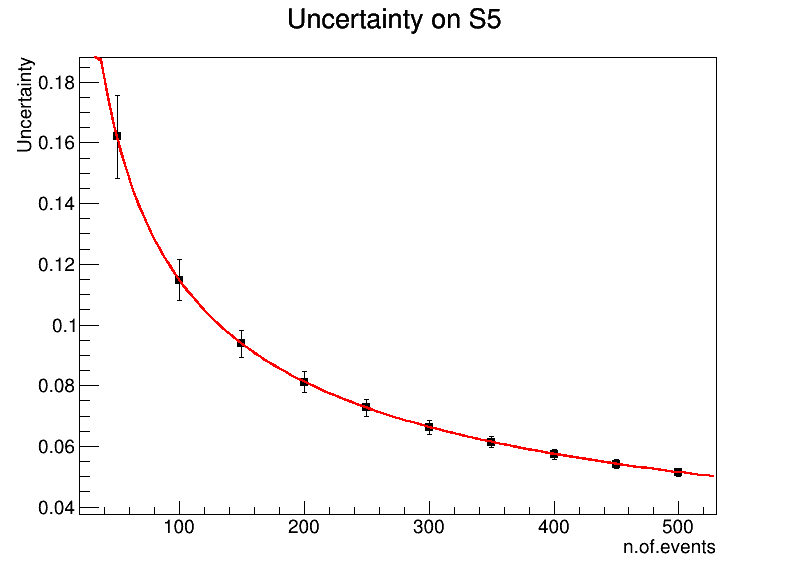
\includegraphics[width=0.45\textwidth]{figs/error-Q2_5_6_S5.png}
            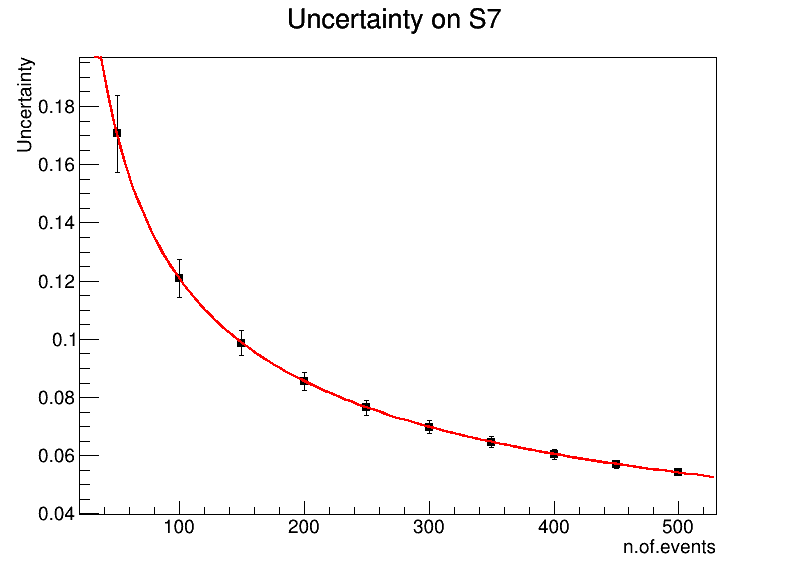
\includegraphics[width=0.45\textwidth]{figs/error-Q2_5_6_S7.png}
            \caption{Uncertainty of the angular observables $S_5$ and $S_7$, extracted from simulated events of the decay $B\to K^*\ell^+\ell^-$ and as a function of the number of simulated events $K$. The red curve represents a fit to the function given in \refeq{unc-on-mean}.}
        \label{fig:errors}
\end{figure}

\hrulefill\\
{\textbf{\color{red}[dvd: can the following be removed?]}
We used the simulated events and fitted a likelihood function to them.
\begin{itemize}
    \item For a small number of simulated events, \danny{$K=?$}, we observe a significant bias in the pull distributions.
    \item For a large number of simulated events, \danny{$K=?$}, the uncertainty of the angular observables is
        smaller compared to the results of the method of moments.
\end{itemize}
todo: compare robustness to likelihood fit when fit doesn't
converge. Why exactly doesn't it converge? What if physics model
wrong, say some angular terms are missing.}
\hrulefill


\section{Conclusion}

We have carried out a combined analytical and numerical study of the method of moments; a method for
the extraction of angular observales from the angular distribution of a generic multi-body process.
We have studied the performance of the method of moments using pseudo data derived from the SM
predctions for one uniangular decay ($B\to K\ell^+\ell^-$) and one triangular decay ($B\to K^*\ell^+\ell^-$).
From this, we find rapid convergence of the joint likelihood of the angular observables towards a multivariate Gaussian.
We draw the conclusion that this method exhibits several benefits in the determination of angular observables when
compared with a maximum-likelihood fit.\\

First, we find no bias in the determinations of the angular observables even for a small number of events.
However, this comes at the expense of a slight increase of the order of $10\%$ for the statistical uncertainty
on the mean.
Second, in the absence of acceptance effects, a determination using the method of moments is correct and unbiased
even when not all aspects of the physical distribution are modelled. This is explicitl shown for the case of
higher partial waveds in multibody final states.
Third, we develop a systematic method for the dertermination of detector acceptance effects that lead to
dilution and mixing of the angular observables. We present a way to calculate the necessary unfolding matrix,
which is only computationally feasible when using the method of moments.\\
Fourth, the fact that the joint distribution of the results is Gaussian allows for an easy transfer of correlation
information to theory analyses.
Last but not least, the resulting distribution arises without additional constraints necessary for the convergence
of some maximum-likelihood fits. Therefore the results can be directly combined with similarly-obtained results from
a different experiment, without the need to remove the constraints of measurements that stem from different experiments.\\

In conclusion, we argue that the method of moments is a competetive alternative to maximum-likelihood fits as long
as angular distributions are involved. We wish to raise the interesting prospect of extending this very method to
applications with non-angular orthogonal bases for the PDF.


\acknowledgments

The work of D.v.D has been supported by the Bundesministerium f\"ur Bildung und Forschung (BMBF).
We would like to thank Ulrik Egede and Konstantinos Petridis for insightful discussions.
\danny{Potential people to read the manuscript: Jochen Dingfelder (Belle-II, Bonn), Ulrik Egede (LHCb, Imperial London), Christoph Langenbruch (LHCb, Warwick), Michel De Cian (LHCb, Heidelberg), Adrian Bevan (ATLAS, Queen Mary)  }
D.v.D would like to thank Gudrun Hiller and Martin Jung for discussing the results of \cite{Das:2014sra} prior to publication.

\appendix

\section{Application to $\bar{B}\to\bar{K}\ell^+\ell^-$}
\label{app:btokll}

The PDF for the decay $\bar{B}\to\bar{K}\ell^+\ell^-$ has been calculated for the most
complete basis of dimension-six $b\to s \ell^+\ell^-$ operators. It reads \cite{Bobeth:2007dw,Bobeth:2012vn}
\begin{equation}
    P(q^2, \cos\theta_1) = \frac{1}{\Gamma} \frac{\rmdx{^4\Gamma}}{\rmdx{q^2} \rmdx{\cos\theta_1}} = \frac{a(q^2)}{\Gamma} + \frac{b(q^2)}{\Gamma} \cos\theta_1 + \frac{c(q^2)}{\Gamma} \cos^2\theta_1 = \sum_i P_i f_i(\cos\theta_1)\,,
\end{equation}
where the basis of angular functions $\lbrace f_i\rbrace$ reads
\begin{equation}
\begin{aligned}
    f_1 & = 1\,, &
    f_2 & = \cos\theta_1\,, &
    f_2 & = \cos^2\theta_1\,.
\end{aligned}
\end{equation}
Here we denote the dilepton mass squared as $q^2$, and the dilepton helicity angle as $\theta_1 \equiv \theta_{\ell}$. We transform the PDF from a $\cos\theta_1$-dependence
to a $\theta_1$-dependence,
\begin{equation}
    P(q^2, \theta_1) = \sum_i P_i f_i(\cos\theta_1) \sin \theta_1\,.
\end{equation}
where we define $P_{\lbrace 1,2,3\rbrace} \equiv \lbrace a, b, c\rbrace / \Gamma$.\\

The dual basis $\lbrace \dual{f}_i\rbrace$ reads
\begin{equation}
\begin{aligned}
    \dual{f}_1 & = \frac{9}{8} - \frac{15}{8}\cos^2\theta_1\,, &
    \dual{f}_2 & = \frac{3}{2}\cos\theta_1\,, &
    \dual{f}_3 & = -\frac{15}{8} + \frac{45}{8}\cos^2\theta_1\,,
\end{aligned}
\end{equation}
such that
\begin{equation}
    \int_0^\pi \rmdx{\theta_1} \dual{f}_i(\theta_1) P(q^2, \theta_1) = S_i(q^2)\,.
\end{equation}

\section{Application to $\bar{B}\to\bar{K}\pi\ell^+\ell^-$ (S-wave and P-wave)}
\label{app:btokstarll}

The PDF for the decay $\bar{B}\to\bar{K}\pi\ell^+\ell^-$ --- up to and including P-wave contributions --- has been calculated
for the most general basis of dimension-six $b\to s$ operators. It reads, expressed in terms of the angular observables $\lbrace J_i\rbrace$ \cite{Blake:2012mb,Bobeth:2012vn}
\begin{equation}
    P(q^2, \cos\theta_1, \cos\theta_2, \theta_3) = \frac{1}{\rmdx{\Gamma}/\rmdx{q^2}} \frac{\rmdx{^4\Gamma}}{\rmdx{q^2} \rmdx{\cos\theta_1} \rmdx{\cos\theta_2} \rmdx{\theta_3}} = \frac{3}{8\pi} \sum_k \frac{J_{k}(q^2)}{\rmdx{\Gamma} /\, \rmdx{q^2}} f_k(\cos\theta_1, \cos\theta_2, \theta_3)\,,
\end{equation}
where $\theta_1 \equiv \theta_\ell$ is the dilepton helicity angle, and $\theta_2 \equiv \theta_{K}$ is the $\bar{K}\pi$ helicity angle, and $\theta_3 \equiv \phi$ is the azimuthal angle.
The $q^2$-differential decay width reads
\begin{equation}
    \frac{\rmdx{\Gamma}}{\rmdx{q^2}} = \frac{\big(3 J_{1c} - J_{2c}\big) + 2\big(3J_{1s} - J_{2s}\big)}{3}\,.
\end{equation}
The angular functions\footnote{%
    We consistently use the label "$i$" to denote angular function and observables that arise
    from interference between S-wave and P-wave amplitudes. Our convention is related to the convention
    of \cite{Bobeth:2012vn} through $f_{1i} \leftrightarrow f_{1sc}$, $f_{2i} \leftrightarrow f_{2sc}$.
} read \cite{Blake:2012mb,Bobeth:2012vn}
\begin{equation}
\begin{aligned}
    f_{1s} & = \sin^2\theta_2 &
    f_{1c} & = \cos^2\theta_2 &
    f_{1i} & = \cos\theta_2\\
    f_{2s} & = \sin^2\theta_2 \cos 2\theta_1 &
    f_{2c} & = \cos^2\theta_2 \cos 2\theta_1 &
    f_{2i} & = \cos\theta_2 \cos 2\theta_1\\
    f_{3}  & = \sin^2\theta_2\sin^2\theta_1 \cos 2\theta_3 &
    f_{4}  & = \sin 2\theta_2 \sin 2\theta_1 \cos\theta_3 &
    f_{4i} & = \sin\theta_2 \sin 2\theta_1 \cos\theta_3\\
    f_{5}  & = \sin 2\theta_2 \sin \theta_1 \cos\theta_3 & & &
    f_{5i} & = \sin\theta_2 \sin \theta_1 \cos\theta_3\\
    f_{6s} & = \sin^2\theta_2 \cos\theta_1 &
    f_{6c} & = \cos^2\theta_2 \cos\theta_1\\
    f_{7}  & = \sin 2\theta_2 \sin \theta_1 \sin\theta_3 & & &
    f_{7i} & = \sin\theta_2 \sin \theta_1 \sin\theta_3\\
    f_{8}  & = \sin 2\theta_2 \sin 2\theta_1 \sin\theta_3 & & &
    f_{8i} & = \sin\theta_2 \sin 2\theta_1 \sin\theta_3\\
    f_{9}  & = \sin^2\theta_2\sin^2\theta_1 \sin 2\theta_3\\
\end{aligned}
\end{equation}
In terms of the angles $\theta_1$ and $\theta_2$, instead of their cosines, the PDF reads
\begin{equation}
    P(q^2, \theta_1, \theta_2, \theta_3) = \frac{3}{8\pi} \sum_k S_k(q^2) f_k(\cos\theta_1, \cos\theta_2, \theta_3) \sin\theta_1 \sin\theta_2\,,
\end{equation}
where we also define $S_k(q^2) \equiv J_k(q^2) / (\rmdx{\Gamma} /\, \rmdx{q^2})$.\\

The dual basis reads
\begin{equation}
\begin{aligned}
    \dual{f}_{1s} & = \frac{\big( 63 \sin^2\theta_2 - 42 \cos^2\theta_2\big) + \big(  45 \sin^2\theta_2 - 30 \cos^2\theta_2\big)\cos 2\theta_1}{64} \,,\\
    \dual{f}_{1c} & = \frac{\big(-21 \sin^2\theta_2 + 84 \cos^2\theta_2\big) + \big( -15 \sin^2\theta_2 + 60 \cos^2\theta_2\big)\cos 2\theta_1}{32} \,,\\
    \dual{f}_{2s} & = \frac{\big( 45 \sin^2\theta_2 - 30 \cos^2\theta_2\big) + \big(+135 \sin^2\theta_2 - 90 \cos^2\theta_2\big)\cos 2\theta_1}{64} \,,\\
    \dual{f}_{2c} & = \frac{\big(-15 \sin^2\theta_2 + 60 \cos^2\theta_2\big) + \big( -45 \sin^2\theta_2 +180 \cos^2\theta_2\big)\cos 2\theta_1}{32} \,,
\end{aligned}
\end{equation}
as well as
\begin{equation}
\begin{aligned}
    \dual{f}_{1i} & = \frac{\big(21 + 15 \cos1\theta_2\big)\cos\theta_2}{16}               \,,&
    \dual{f}_{2i} & = \frac{\big(15 + 45 \cos1\theta_2\big)\cos\theta_2}{16}               \,,\\
    \dual{f}_{3}  & = \frac{75 \sin^2\theta_2 \sin^2\theta_1 \cos2\theta_3}{32}                \,,& &\\
    \dual{f}_{4}  & = \frac{75 \sin 2\theta_2 \sin 2\theta_1 \cos \theta_3}{32}                \,,&
    \dual{f}_{4i} & = \frac{15 \sin  \theta_2 \sin 2\theta_1 \cos \theta_3}{8}                 \,,\\
    \dual{f}_{5}  & = \frac{15 \sin 2\theta_2 \sin  \theta_1 \cos \theta_3}{8}                 \,,&
    \dual{f}_{5i} & = \frac{3  \sin  \theta_2 \sin  \theta_1 \cos \theta_3}{2}                 \,,\\
    \dual{f}_{6s} & = \frac{\big( 9\sin^2\theta_2 -  6 \cos^2\theta_2\big)\cos\theta_1}{4} \,,&
    \dual{f}_{6c} & = \frac{\big(-3\sin^2\theta_2 + 12 \cos^2\theta_2\big)\cos\theta_1}{2} \,,\\
    \dual{f}_{7}  & = \frac{15 \sin 2\theta_2 \sin  \theta_1 \sin \theta_3}{8}                 \,,&
    \dual{f}_{7i} & = \frac{3  \sin  \theta_2 \sin  \theta_1 \sin \theta_3}{2}                 \,,\\
    \dual{f}_{8}  & = \frac{75 \sin 2\theta_2 \sin 2\theta_1 \sin \theta_3}{32}                \,,&
    \dual{f}_{8i} & = \frac{15 \sin  \theta_2 \sin 2\theta_1 \sin \theta_3}{8}                 \,,\\
    \dual{f}_{9}  & = \frac{75 \sin^2\theta_2 \sin^2\theta_1 \sin2\theta_3}{32}                \,.\\
\end{aligned}
\end{equation}
such that
\begin{equation}
    \int_0^\pi \rmdx{\theta_1} \int_0^\pi \rmdx{\theta_2} \int_0^{2\pi} \rmdx{\theta_3} \dual{f}_k(\theta_1,\theta_2,\theta_3) P(q^2, \theta_1,\theta_2,\theta_3) = S_k(q^2)\,.
\end{equation}

\section{Application to $\bar{B}\to P_1 P_2\ell^+\ell^-$ (all partial waves)}
\label{app:btokpill}

The class of semileptonic $\bar{B}\to P_1 P_2 \ell_1\bar\ell_2$ decays, where $P_1$, and $P_2$ are pseudoscalar mesons,
and $\ell_1$ and $\bar\ell_2$ are charged or neutral leptons, includes decays
such as $\bar{B}\to\bar{K}\pi\ell^+\ell^-$ and $\bar{B}\to \pi\pi\ell^-\bar\nu_\ell$.
Their decay PDFs can generally be written as \cite{Lee:1992ih}
\begin{equation}
    P(q^2, p^2, \cos\theta_1, \cos \theta_2, \theta_3) = \frac{1}{\langle \Gamma\rangle}\frac{\rmdx{^5 \Gamma}}{\rmdx{q^2} \rmdx{p^2} \rmdx{\cos\theta_1} \rmdx{\cos\theta_2} \rmdx{\theta_3}} = \frac{1}{4\pi} \sum_k \frac{I_k(q^2, p^2, \cos\theta_2)}{\Gamma} f_k(\cos\theta_1,\theta_3)\,,
\end{equation}
where
\begin{equation}
\begin{aligned}
    f_1 & = 1\,,              &
    f_2 & = \cos 2\theta_1\,, &
    f_3 & = \sin^2\theta_1 \cos 2\theta_3\,,\\
    f_4 & = \sin 2\theta_1 \cos  \theta_3\,,&
    f_5 & = \sin  \theta_1 \cos  \theta_3\,,&
    f_6 & = \cos  \theta_1\,, \\
    f_7 & = \sin  \theta_1 \sin  \theta_3\,,&
    f_8 & = \sin 2\theta_1 \sin  \theta_3\,,&
    f_9 & = \sin^2\theta_1 \sin 2\theta_3\,.\\
\end{aligned}
\end{equation}
Here we denote dilepton mass squared and the dilepton helicity angle as $q^2$ and $\theta_1$, while
the dimeson mass squared and the dimeson helicity angles are denoted as $p^2$ and $\theta_2$. The
azimuthal angle is denoted as $\theta_3$.
The total decay width is
\begin{equation}
    \langle \Gamma\rangle = \int_0^\pi \rmdx{\theta_2} \rmdx{q^2} \rmdx{p^2} \sin\theta_2 \frac{3I_1(q^2, p^2, \cos\theta_2) - I_2(q^2, p^2, \cos\theta_2)}{3}\,.
\end{equation}
As previous, we transform from a $\cos\theta_2$-dependence to a $\theta_2$-dependence.
\begin{equation}
\begin{aligned}
    P(q^2, p^2, \theta_1, \theta_2, \theta_3)
    & = \frac{1}{4\pi} \sum_k \frac{I_k(q^2, p^2, \cos\theta_2)}{\Gamma} f_i(\theta_1, \theta_3) \sin\theta_1 \sin\theta_2\\
    & \equiv \frac{1}{4\pi} \sum_k S_k(q^2, p^2, \theta_2) f_k(\theta_1, \theta_3) \sin\theta_1\,.
\end{aligned}
\end{equation}
where we also define $S_k(q^2, p^2, \theta_2) \equiv \sin\theta_2 I_k(q^2, p^2, \cos\theta_2) / \langle \Gamma\rangle$.\\

The dual basis reads
\begin{equation}
\begin{aligned}
    \dual{f}_1 & = \frac{21 + 15 \cos 2\theta_1}{16}\,, &
    \dual{f}_2 & = \frac{15 + 45 \cos 2\theta_1}{16}\,, &
    \dual{f}_3 & = \frac{15}{4} \sin^2\theta_1 \cos 2\theta_3     \,,\\
    \dual{f}_4 & = \frac{15}{4} \sin 2\theta_1 \cos  \theta_3     \,, &
    \dual{f}_5 & = 3            \sin  \theta_1 \cos  \theta_3     \,, &
    \dual{f}_6 & = 3 \cos\theta_1                   \,,\\
    \dual{f}_7 & = 3            \sin  \theta_1 \sin  \theta_3     \,, &
    \dual{f}_8 & = \frac{15}{4} \sin 2\theta_1 \sin  \theta_3     \,, &
    \dual{f}_9 & = \frac{15}{4} \sin^2\theta_1 \sin 2\theta_3     \,.\\
\end{aligned}
\end{equation}
such that
\begin{equation}
    \int_0^\pi \rmdx{\theta_1} \int_0^{2\pi} \rmdx{\theta_3} \dual{f}_i(\theta_1,\theta_3) P(q^2, k^2, \theta_1,\theta_2,\theta_3) = S_i(q^2, k^2, \theta_2)\,.
\end{equation}


\section{Application to $\Lambda_b\to \Lambda(\to N \pi)\ell^+\ell^-$}
\label{app:lambdabtolambdall}

The PDF for the decay --- in the presence of Standard-Model operators and their chirality-flipped counter parts --- reads \cite{Boeer:2014xx}
\begin{equation}
    P(q^2, \cos\theta_1, \cos\theta_2, \theta_3) = \frac{1}{\rmdx{\Gamma} /\, \rmdx{q^2}} \frac{\rmdx{^4\Gamma}}{\rmdx{q^2} \rmdx{\cos\theta_1} \rmdx{\cos\theta_2} \rmdx{\theta_3}} = \frac{3}{8\pi} \sum_i \frac{K_{i}(q^2)}{\rmdx{\Gamma} /\, \rmdx{q^2}} f_i(\cos\theta_1, \cos\theta_2, \theta_3)\,,
\end{equation}
where $q^2$ denotes the dilepton mass squared, $\theta_1 \equiv \theta_\ell$ and $\theta_2 \equiv \theta_\Lambda$ denote the
helicity angles in the dilepton and
$N\pi$ systems, respectively, and $\theta_3 = \phi$ denotes the azimuthal angle.
The basis of angular functions reads \cite{Boeer:2014xx}
\begin{equation}
    \begin{aligned}
% 1
        f_{1ss} & = \sin^2\theta_1 &
        f_{1cc} & = \cos^2\theta_1 &
        f_{1c}  & = \cos\theta_1\\
% 2
        f_{2ss} & = \sin^2\theta_1 \cos\theta_2 &
        f_{2cc} & = \cos^2\theta_1 \cos\theta_2 &
        f_{2c}  & = \cos\theta_1   \cos\theta_2 \\
% 3
        f_{3sc} & = \sin\theta_1 \cos\theta_1 \sin\theta_2 \cos\theta_3 &
        f_{3s}  & = \sin\theta_1              \sin\theta_2 \cos\theta_3 \\
% 4
        f_{4sc} & = \sin\theta_1 \cos\theta_1 \sin\theta_2 \sin\theta_3 &
        f_{4s}  & = \sin\theta_1              \sin\theta_2 \sin\theta_3
    \end{aligned}
\end{equation}
The decay width reads
\begin{equation}
    \frac{\rmdx{\Gamma}} {\rmdx{q^2}} = 2 K_{1ss} + K_{1cc}
\end{equation}
In terms of the angles $\theta_1$ and $\theta_2$, instead of the cosines, the PDF reads
\begin{equation}
    P(q^2, \theta_1, \theta_2, \theta_3) = \frac{3}{8\pi} \sum_i S_i(q^2) f_i(\cos\theta_1, \cos\theta_2, \theta_3) \sin\theta_1 \sin\theta_2\,,
\end{equation}
where we also define $S_i(q^2) \equiv K_i(q^2) / (\rmdx{\Gamma} /\, \rmdx{q^2})$.\\

The dual basis reads
\begin{equation}
    \begin{aligned}
% 1
        \dual f_{1ss} & = \frac{1}{4}\big(3 \sin^2\theta_1 - 2 \cos^2\theta_1\big) &
        \dual f_{1cc} & = \frac{1}{2}\big(- \sin^2\theta_1 + 4 \cos^2\theta_1\big) &
        \dual f_{1c}  & = \cos\theta_1\\
% 2
        \dual f_{2ss} & = \frac{3}{4}\big(3 \sin^2\theta_1 - 2 \cos^2\theta_1\big) \cos\theta_2 &
        \dual f_{2cc} & = \frac{3}{2}\big(- \sin^2\theta_1 + 4 \cos^2\theta_1\big) \cos\theta_2 &
        \dual f_{2c}  & = 3 \cos\theta_1   \cos\theta_2 \\
% 3
        \dual f_{3sc} & = \frac{15}{2}\sin\theta_1 \cos\theta_1 \sin\theta_2 \cos\theta_3 &
        \dual f_{3s}  & = \frac{3}{2} \sin\theta_1              \sin\theta_2 \cos\theta_3 \\
% 4
        \dual f_{4sc} & = \frac{15}{2}\sin\theta_1 \cos\theta_1 \sin\theta_2 \sin\theta_3 &
        \dual f_{4s}  & = \frac{3}{2} \sin\theta_1              \sin\theta_2 \sin\theta_3
    \end{aligned}
\end{equation}
such that
\begin{equation}
    \int_0^\pi \rmdx{\theta_1} \int_0^\pi \rmdx{\theta_2} \int_0^{2\pi} \rmdx{\theta_3} P(q^2, \theta_1, \theta_2, \theta_3) \dual{f}_i(\theta_1, \theta_2, \theta_3) = S_i(q^2)\,.
\end{equation}


\section{On the Partial-Wave Expansions of Angular Observables}
\label{app:partial-waves}

Let $S \equiv S(\vec{\nu},\theta)$ be an observable of only one angle $\theta$ and further non-angular variables $\vec{\nu}$. \fred{This is confusing: in the intro, we define $S$ as independent of any angle.} \fred{What about two angles? More amplitudes seem trivial, one would just have more $S_i$} Further, let
$S$ have an expansion in terms of partial waves $l_1, l_2 = 0,1,2,\dots \hat{=}$ S,P,D$,\dots$ of the underlying amplitudes $A_1$ and $A_2$,
\begin{equation}
    \label{eq:def-partial-wave-observable}
    S(\theta) \equiv F\left[A_1(\theta) A_2^*(\theta)\right] \equiv F\left[\left(\sum_{l_1=0}^\infty A_1^{(l_1)} p_{l_1}^{(m_1)}(\cos\theta)\right) \left(\sum_{l_2=0}^\infty A_2^{*(l_2)} p_{l_2}^{(m_2)}(\cos\theta)\right)\right]\,,
\end{equation}
where $F \in \{\text{Re},\text{Im}\}$ denotes taking either the real
or the imaginary part. \fred{Now $\nuvec$ gone}
$p_{l}^{(m)}$ is an \emph{associated Legendre} polynomial and $m_i$ is the third component of the angular momentum of the amplitude $A_i$, and we impose $m_1 \geq m_2$.\\

From the positivity of amplitudes, one immediately finds
\begin{equation}
    \int \rmdx{\cos\theta}  \, |A_i(\theta)|^2 = \sum_{l_i = 0}^\infty |A_i^{(l_i)}|^2 n_{l_i, m_i} < \infty\,,
\end{equation}
where we introduce $n_{l,m}$ via the scalar product of two associated Legendre polynomials,
\begin{equation}
    \label{eq:legendre-scalar-product}
    n_{l, m} \delta_{l, l'} \equiv \int_{-1}^1 \rmdx{\cos\theta} p_{l}^{(m)}(\cos\theta) p_{l'}^{(m)} (\cos\theta)  = \frac{2}{(2 l + 1)} \frac{(l + m)!}{(l - m)!} \delta_{l, l'}\,.
\end{equation}
Using the large-$l$ behaviour of $n_{l,m}$ one finds that with increasing $l_i$ the partial-wave amplitudes must asymptotically fall off as \fred{Let's say why. Unitarity?}
\begin{equation}
    |A_i^{(l_i)}(\cos\theta)| \Big|_{l_i \gg m_i} \sim \frac{1}{\sqrt{l_i}}\,.
\end{equation}
This motivates to cut the partial-wave expansion off at some angular momentum $L$.\\

Will will show in the following that such a cut off
is compatible with defining a basis of angular observables as coefficients of Legendre polynomials in $\cos\theta$. Since this expansion implies
a well defined total angular momentum for each observable, one ensures that the observables can in fact be disentangled experimentally.\\

We propose the decomposition of $S$ in terms of the associated Legendre polynomials $p_{j}^{(m)}(\cos\theta)$, with total angular momentum $j$ and its third component $m=m_1 + m_2$.
\begin{equation}
    S(\vec{\nu}, \theta) = \sum_j S_{j,m}(\vec{\nu}) p_{j}^{(m)}(\cos\theta)\,.
\end{equation}
This parametrization has two merits. First, we can immediately project out the angular observables $S_{j,m}$ by means of \refeq{legendre-scalar-product}:
\begin{equation}
    S_{j,m}(\vec{\nu}) = \frac{1}{n_{j,m}} \int_{-1}^{+1} \rmdx{\cos\theta} S(\vec{\nu},\cos \theta) p_{j}^{(m)}(\cos\theta)\,.
\end{equation}
(Here and in the next step we may exchage the integral and the
series because each element of the series is a product of
polynomials on the compact support [-1,1], and thus each integral
is absolutely convergent).
Second, we can immediately express $S_{j,m}(\vec{\nu})$ in terms of
the partial-wave amplitudes,
\begin{equation}
    \label{eq:partial-wave-observable-infinite}
    \begin{aligned}
        S_{j,m}(\vec{\nu})
            & = \frac{1}{n_{j,m}} \int_{-1}^{+1} \rmdx{\cos\theta} p_{j}^{(m_1 + m_2)}(\cos\theta) \sum_{l_1,l_2=0}^\infty F\left[A_{1}^{l_1} p_{l_1}^{(m_1)}(\cos\theta) A_{2}^{*(l_2)}p_{l_2}^{(m_2)}(\cos\theta)\right]\\
            & = \sum_{l_1,l_2=0}^\infty F\left[A_{1}^{l_1} A_{2}^{*(l_2)}\right] \frac{T_{l_1,l_2,j}^{(m_1,m_2)}}{n_{j,m}}\,,\qquad\text{with }m = m_1 + m_2\,.
    \end{aligned}
\end{equation}

In the last step, we use Gaunt's formula \cite{Gaunt:1929} to integrate a triple product of associated Legendre polynomials,
\begin{equation}
\begin{aligned}
    T_{l_1,l_2,j}^{(m_1,m_2)}
        & = \int_{-1}^{+1} \rmdx{\cos\theta} p_{j}^{(m_1 + m_2)}(\cos\theta) p_{l_1}^{(m_1)}(\cos\theta) p_{l_2}^{(m_2)}(\cos\theta)\\
        & = (-1)^{s - l_1 - m_2} \frac{2 (l_1 + m_1)! (l_2 + m_2)! (2s - 2 l_2)! s!}{(l_1 - m_1)! (s - j)! (s - l_1)! (s - l_2)! (2s + 1)!}\\
        & \times \sum_{t=p}^q (-1)^t \frac{(j + m + t)!(l_1 + l_2 - m - t)!}{t! (j - m - t)! (l_1 - l_2 + m + t)! (l_2 - m_2 - t)!}\,,
\end{aligned}
\end{equation}
where
\begin{equation}
\begin{aligned}
    m & = m_1 + m_2\,, &
    m_1 & \geq m_2\,,  \\
    j, l_1, l_2 & \geq 0\,, &
    m, m_1, m_2 & \geq 0\,,
\end{aligned}
\end{equation}
and
\begin{equation}
\begin{aligned}
    s & = \frac{j + l_1 + l_2}{2}\,, &
    p & = \max(0, l_2 - l_1 - m)\,, &
    q & = \min(l_1 + l_2 - m, j - m, l_2 - m_2)\,.
\end{aligned}
\end{equation}
The necessary conditions for $T \neq 0$ are
\begin{equation}
    \label{eq:angular-momentum-addition}
    s \in \mathbb{N}\qquad \wedge \qquad l_1 - l_2 \leq l \leq l_1 + l_2,.
\end{equation}
The latter condition is well known from adding angular momenta. Note, however, that
the sum in \refeq{def-partial-wave-observable} goes to infinitely high angular momenta $l_1$ and $l_2$. As a consequence
of this and of \refeq{angular-momentum-addition}, the angular observables $P_{j,m}$
consist of sums with infinitely many terms. It is then up to theoretical analyses to
estimate or calculate the impact of individual contributions, with or without the cut off $L$.
For such an analysis in the decay $B\to K\pi\ell^+\ell^-$ we refer to \cite{Das:2014sra}.
We close by remarking that for any angular-momentum cut off $l < L$\fred{Do you mean $L < \infty$?}, one can find an upper limit for the squared sum
of all remaining partial waves through the inclusive decay; i.e., schematically
\begin{equation}
    \sum_{i=1}^2 \sum_{l=L}^\infty |A_i^{(l)}|^2 \leq \frac{\rmdx{^{1 + \dim\vec\nu}} \Gamma_\text{incl}}{\rmdx{\cos\theta} \rmdx{\vec\nu}}\,.
\end{equation}


\bibliography{references}

\end{document}
